{\color{indiagreen}\subsection{Ohmov zakon}}
\begin{align*}
	{\color{bostonuniversityred}U} &= {\color{bostonuniversityred}RI}\\
	R &\dots \text{upor \textbf{če upor ni konstanten ohmov zakon ne velja}}\\
	{\color{bostonuniversityred}R} &= {\color{bostonuniversityred}\frac{U}{I}}[1\frac{V}{A} = 1\Omega]\\
\end{align*}

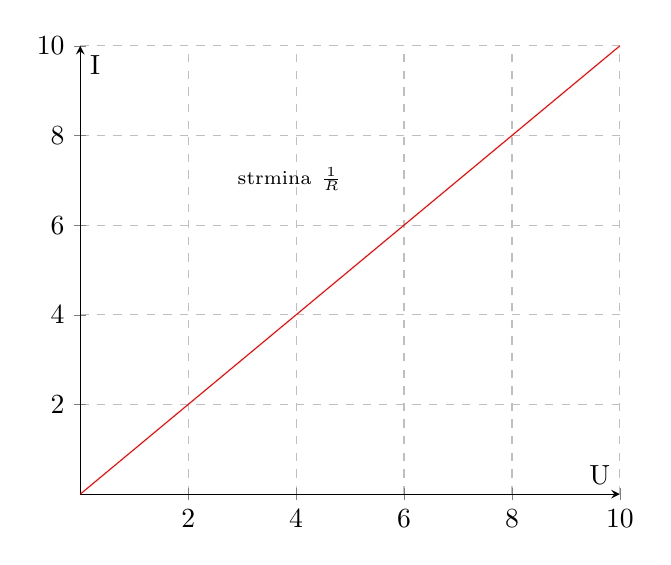
\begin{tikzpicture}
	\begin{axis}[
	    xlabel={U},
	    ylabel={I},
	    xmin=0, xmax=10,
	    ymin=-0, ymax=10,
	    xtick={0,2,4,6,8,10},
	    ytick={0,2,4,6,8,10},
	    ymajorgrids=true,
	    xmajorgrids=true,
	    grid style=dashed,
	    axis lines=middle,
	]
	\addplot[domain=0:10,red] {x};

	\end{axis}
	\node[text width=2cm] at (3,4){\scriptsize {strmina $\frac{1}{R}$}};
\end{tikzpicture}
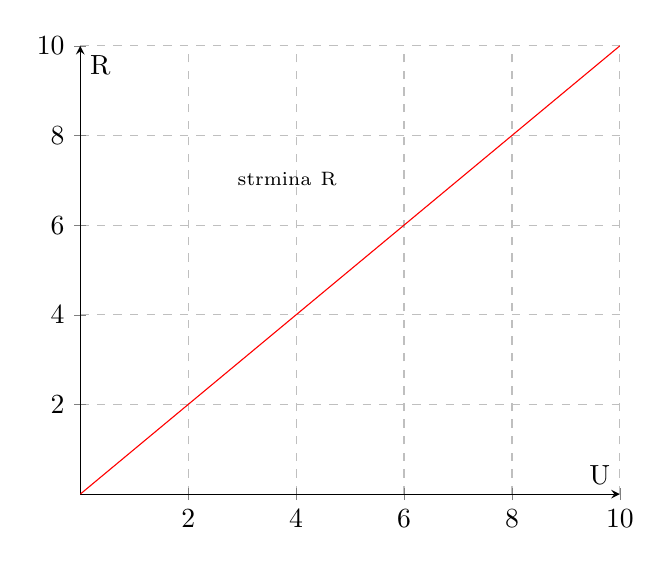
\begin{tikzpicture}
	\begin{axis}[
	    xlabel={U},
	    ylabel={R},
	    xmin=0, xmax=10,
	    ymin=-0, ymax=10,
	    xtick={0,2,4,6,8,10},
	    ytick={0,2,4,6,8,10},
	    ymajorgrids=true,
	    xmajorgrids=true,
	    grid style=dashed,
	    axis lines=middle,
	]
	\addplot[domain=0:10,red] {x};

	\end{axis}
	\node[text width=2cm] at (3,4){\scriptsize {strmina R}};
\end{tikzpicture}\\
Z višanjem temperature se upornost veča in posledično je manjši tok.\\
\textbf{Žarnica}\\
\begin{tikzpicture}
	\begin{axis}[
	    xlabel={I},
	    ylabel={U},
	    xmin=0, xmax=10,
	    ymin=-0, ymax=10,
	    xtick={0,2,4,6,8,10},
	    ytick={0,2,4,6,8,10},
	    ymajorgrids=true,
	    xmajorgrids=true,
	    grid style=dashed,
	    axis lines=middle,
	]
	\addplot[domain=0:10,red] {(7*x+1)^(1/2)-1};
	\end{axis}
\end{tikzpicture}\\
Večja je temperatura, večji je upor, manjši je tok.\\
\textbf{Za generator(vir napetosti)}\\
\begin{align*}
	{\color{bostonuniversityred}U} &= {\color{bostonuniversityred}U_g - R_n I}\\ 
	U_g &\dots \text{Gonilna napetost}\\
	R_n &\dots \text{Notranji upor generatorja}\\
\end{align*}
